\chapter{Thao tác bit}

Tất cả dữ liệu trong các chương trình máy tính được lưu trữ nội bộ dưới dạng các bit,
tức là dưới dạng các số 0 và 1.
Chương này thảo luận về biểu diễn bit
của các số nguyên, và trình bày các ví dụ
về cách sử dụng các phép toán bit.
Hóa ra có rất nhiều ứng dụng cho
việc thao tác bit trong lập trình thuật toán.

\section{Biểu diễn bit}

\index{bit representation}

Trong lập trình, một số nguyên $n$ bit được lưu trữ nội bộ
dưới dạng một số nhị phân bao gồm $n$ bit.
Ví dụ, kiểu dữ liệu \texttt{int} trong C++ là
một kiểu 32 bit, có nghĩa là mọi số \texttt{int}
bao gồm 32 bit.

Đây là biểu diễn bit của
số \texttt{int} 43:
\[00000000000000000000000000101011\]
Các bit trong biểu diễn được đánh chỉ số từ phải sang trái.
Để chuyển đổi một biểu diễn bit $b_k \cdots b_2 b_1 b_0$ thành một số,
chúng ta có thể sử dụng công thức
\[b_k 2^k + \ldots + b_2 2^2 + b_1 2^1 + b_0 2^0.\]
Ví dụ,
\[1 \cdot 2^5 + 1 \cdot 2^3 + 1 \cdot 2^1 + 1 \cdot 2^0 = 43.\]

Biểu diễn bit của một số có thể là
\key{có dấu (signed)} hoặc \key{không dấu (unsigned)}.
Thường thì một biểu diễn có dấu được sử dụng,
có nghĩa là cả số âm và số dương
đều có thể được biểu diễn.
Một biến có dấu $n$ bit có thể chứa bất kỳ
số nguyên nào trong khoảng từ $-2^{n-1}$ đến $2^{n-1}-1$.
Ví dụ, kiểu \texttt{int} trong C++ là
một kiểu có dấu, vì vậy một biến \texttt{int} có thể chứa bất kỳ
số nguyên nào trong khoảng từ $-2^{31}$ đến $2^{31}-1$.

Bit đầu tiên trong một biểu diễn có dấu
là dấu của số (0 cho các số không âm
và 1 cho các số âm), và
$n-1$ bit còn lại chứa độ lớn của số.
\key{Bù hai (Two's complement)} được sử dụng, có nghĩa là
số đối của một số được tính bằng cách đầu tiên
đảo tất cả các bit trong số đó,
và sau đó tăng số đó lên một.

Ví dụ, biểu diễn bit của
số \texttt{int} $-43$ là
\[11111111111111111111111111010101.\]

Trong một biểu diễn không dấu, chỉ có các số không âm
mới có thể được sử dụng, nhưng giới hạn trên cho các giá trị lớn hơn.
Một biến không dấu $n$ bit có thể chứa bất kỳ
số nguyên nào trong khoảng từ $0$ đến $2^n-1$.
Ví dụ, trong C++, một biến \texttt{unsigned int}
có thể chứa bất kỳ số nguyên nào trong khoảng từ $0$ đến $2^{32}-1$.

Có một mối liên hệ giữa các
biểu diễn:
một số có dấu $-x$ bằng một số không dấu $2^n-x$.
Ví dụ, đoạn mã sau cho thấy
số có dấu $x=-43$ bằng số không dấu
$y=2^{32}-43$:
\begin{lstlisting}
int x = -43;
unsigned int y = x;
cout << x << "\n"; // -43
cout << y << "\n"; // 4294967253
\end{lstlisting}

Nếu một số lớn hơn giới hạn trên
của biểu diễn bit, số đó sẽ bị tràn.
Trong một biểu diễn có dấu,
số tiếp theo sau $2^{n-1}-1$ là $-2^{n-1}$,
và trong một biểu diễn không dấu,
số tiếp theo sau $2^n-1$ là $0$.
Ví dụ, hãy xem xét đoạn mã sau:
\begin{lstlisting}
int x = 2147483647
cout << x << "\n"; // 2147483647
x++;
cout << x << "\n"; // -2147483648
\end{lstlisting}

Ban đầu, giá trị của $x$ là $2^{31}-1$.
Đây là giá trị lớn nhất có thể được lưu trữ
trong một biến \texttt{int},
vì vậy số tiếp theo sau $2^{31}-1$ là $-2^{31}$.


\section{Các phép toán bit}

\newcommand\XOR{\mathbin{\char`\^}}

\subsubsection{Phép toán And}

\index{and operation}

Phép toán \key{and} $x$ \& $y$ tạo ra một số
có các bit một ở những vị trí mà cả
$x$ và $y$ đều có bit một.
Ví dụ, $22$ \& $26$ = 18, bởi vì

\begin{center}
\begin{tabular}{rrr}
& 10110 & (22)\\
\& & 11010 & (26) \\
\hline
 = & 10010 & (18) \\
\end{tabular}
\end{center}

Sử dụng phép toán and, chúng ta có thể kiểm tra xem một số
$x$ có phải là số chẵn hay không vì
$x$ \& $1$ = 0 nếu $x$ chẵn, và
$x$ \& $1$ = 1 nếu $x$ lẻ.
Tổng quát hơn, $x$ chia hết cho $2^k$
chính xác khi $x$ \& $(2^k-1)$ = 0.

\subsubsection{Phép toán Or}

\index{or operation}

Phép toán \key{or} $x$ | $y$ tạo ra một số
có các bit một ở những vị trí mà ít nhất một trong
$x$ và $y$ có bit một.
Ví dụ, $22$ | $26$ = 30, bởi vì

\begin{center}
\begin{tabular}{rrr}
& 10110 & (22)\\
| & 11010 & (26) \\
\hline
 = & 11110 & (30) \\
\end{tabular}
\end{center}

\subsubsection{Phép toán Xor}

\index{xor operation}

Phép toán \key{xor} $x$ $\XOR$ $y$ tạo ra một số
có các bit một ở những vị trí mà chính xác một trong
$x$ và $y$ có bit một.
Ví dụ, $22$ $\XOR$ $26$ = 12, bởi vì

\begin{center}
\begin{tabular}{rrr}
& 10110 & (22)\\
$\XOR$ & 11010 & (26) \\
\hline
 = & 01100 & (12) \\
\end{tabular}
\end{center}

\subsubsection{Phép toán Not}

\index{not operation}

Phép toán \key{not} \textasciitilde$x$
tạo ra một số trong đó tất cả các bit của $x$
đã được đảo ngược.
Công thức \textasciitilde$x = -x-1$ đúng,
ví dụ, \textasciitilde$29 = -30$.

Kết quả của phép toán not ở cấp độ bit
phụ thuộc vào độ dài của biểu diễn bit,
bởi vì phép toán đảo ngược tất cả các bit.
Ví dụ, nếu các số là các số
\texttt{int} 32 bit, kết quả như sau:

\begin{center}
\begin{tabular}{rrrr}
$x$ & = & 29 &   00000000000000000000000000011101 \\
\textasciitilde$x$ & = & $-30$ & 11111111111111111111111111100010 \\
\end{tabular}
\end{center}

\subsubsection{Phép dịch bit}

\index{bit shift}

Phép dịch bit trái $x < < k$ nối thêm $k$
bit không vào số,
và phép dịch bit phải $x > > k$
loại bỏ $k$ bit cuối cùng khỏi số.
Ví dụ, $14 < < 2 = 56$,
bởi vì $14$ và $56$ tương ứng với 1110 và 111000.
Tương tự, $49 > > 3 = 6$,
bởi vì $49$ và $6$ tương ứng với 110001 và 110.

Lưu ý rằng $x < < k$
tương ứng với việc nhân $x$ với $2^k$,
và $x > > k$
tương ứng với việc chia $x$ cho $2^k$
làm tròn xuống thành một số nguyên.

\subsubsection{Ứng dụng}

Một số có dạng $1 < < k$ có một bit một
ở vị trí $k$ và tất cả các bit khác là không,
vì vậy chúng ta có thể sử dụng các số như vậy để truy cập các bit đơn lẻ của các số.
Cụ thể, bit thứ $k$ của một số là một
chính xác khi $x$ \& $(1 < < k)$ khác không.
Đoạn mã sau in ra biểu diễn bit
của một số \texttt{int} $x$:

\begin{lstlisting}
for (int i = 31; i >= 0; i--) {
    if (x&(1<<i)) cout << "1";
    else cout << "0";
}
\end{lstlisting}

Cũng có thể sửa đổi các bit đơn lẻ
của các số bằng cách sử dụng các ý tưởng tương tự.
Ví dụ, công thức $x$ | $(1 < < k)$
đặt bit thứ $k$ của $x$ thành một,
công thức
$x$ \& \textasciitilde $(1 < < k)$
đặt bit thứ $k$ của $x$ thành không,
và công thức
$x$ $\XOR$ $(1 < < k)$
đảo bit thứ $k$ của $x$.

Công thức $x$ \& $(x-1)$ đặt bit
một cuối cùng của $x$ thành không,
và công thức $x$ \& $-x$ đặt tất cả các
bit một thành không, ngoại trừ bit một cuối cùng.
Công thức $x$ | $(x-1)$
đảo tất cả các bit sau bit một cuối cùng.
Cũng lưu ý rằng một số dương $x$ là
một lũy thừa của hai chính xác khi $x$ \& $(x-1) = 0$.

\subsubsection*{Các hàm bổ sung}

Trình biên dịch g++ cung cấp các
hàm sau để đếm bit:

\begin{itemize}
\item
$\texttt{\_\_builtin\_clz}(x)$:
số lượng các số không ở đầu số
\item
$\texttt{\_\_builtin\_ctz}(x)$:
số lượng các số không ở cuối số
\item
$\texttt{\_\_builtin\_popcount}(x)$:
số lượng các số một trong số
\item
$\texttt{\_\_builtin\_parity}(x)$:
tính chẵn lẻ (chẵn hay lẻ) của số lượng các số một
\end{itemize}
\begin{samepage}

Các hàm có thể được sử dụng như sau:
\begin{lstlisting}
int x = 5328; // 00000000000000000001010011010000
cout << __builtin_clz(x) << "\n"; // 19
cout << __builtin_ctz(x) << "\n"; // 4
cout << __builtin_popcount(x) << "\n"; // 5
cout << __builtin_parity(x) << "\n"; // 1
\end{lstlisting}
\end{samepage}

Trong khi các hàm trên chỉ hỗ trợ các số \texttt{int},
cũng có các phiên bản \texttt{long long} của
các hàm có sẵn với hậu tố \texttt{ll}.

\section{Biểu diễn tập hợp}

Mọi tập hợp con của một tập hợp
$\{0,1,2,\ldots,n-1\}$
có thể được biểu diễn dưới dạng một số nguyên $n$ bit
mà các bit một của nó chỉ ra những
phần tử nào thuộc về tập hợp con đó.
Đây là một cách hiệu quả để biểu diễn các tập hợp,
bởi vì mỗi phần tử chỉ yêu cầu một bit bộ nhớ,
và các phép toán tập hợp có thể được triển khai dưới dạng các phép toán bit.

Ví dụ, vì \texttt{int} là một kiểu 32 bit,
một số \texttt{int} có thể biểu diễn bất kỳ tập hợp con nào
của tập hợp $\{0,1,2,\ldots,31\}$.
Biểu diễn bit của tập hợp $\{1,3,4,8\}$ là
\[00000000000000000000000100011010,\]
tương ứng với số $2^8+2^4+2^3+2^1=282$.

\subsubsection{Triển khai tập hợp}

Đoạn mã sau khai báo một biến \texttt{int}
$x$ có thể chứa
một tập hợp con của $\{0,1,2,\ldots,31\}$.
Sau đó, đoạn mã thêm các phần tử 1, 3, 4 và 8
vào tập hợp và in ra kích thước của tập hợp.
\begin{lstlisting}
int x = 0;
x |= (1<<1);
x |= (1<<3);
x |= (1<<4);
x |= (1<<8);
cout << __builtin_popcount(x) << "\n"; // 4
\end{lstlisting}
Sau đó, đoạn mã sau in ra tất cả các
phần tử thuộc về tập hợp:
\begin{lstlisting}
for (int i = 0; i < 32; i++) {
    if (x&(1<<i)) cout << i << " ";
}
// output: 1 3 4 8
\end{lstlisting}

\subsubsection{Các phép toán tập hợp}

Các phép toán tập hợp có thể được triển khai như sau dưới dạng các phép toán bit:

\begin{center}
\begin{tabular}{lll}
& cú pháp tập hợp & cú pháp bit \\
\hline
giao & $a \cap b$ & $a$ \& $b$ \\
hợp & $a \cup b$ & $a$ | $b$ \\
phần bù & $\bar a$ & \textasciitilde$a$ \\
hiệu & $a \setminus b$ & $a$ \& (\textasciitilde$b$) \\
\end{tabular}
\end{center}

Ví dụ, đoạn mã sau đầu tiên xây dựng
các tập hợp $x=\{1,3,4,8\}$ và $y=\{3,6,8,9\}$,
và sau đó xây dựng tập hợp $z = x \cup y = \{1,3,4,6,8,9\}$:

\begin{lstlisting}
int x = (1<<1)|(1<<3)|(1<<4)|(1<<8);
int y = (1<<3)|(1<<6)|(1<<8)|(1<<9);
int z = x|y;
cout << __builtin_popcount(z) << "\n"; // 6
\end{lstlisting}

\subsubsection{Lặp qua các tập hợp con}

Đoạn mã sau duyệt qua
các tập hợp con của $\{0,1,\ldots,n-1\}$:

\begin{lstlisting}
for (int b = 0; b < (1<<n); b++) {
    // xu ly tap hop con b
}
\end{lstlisting}
Đoạn mã sau duyệt qua
các tập hợp con có đúng $k$ phần tử:
\begin{lstlisting}
for (int b = 0; b < (1<<n); b++) {
    if (__builtin_popcount(b) == k) {
        // xu ly tap hop con b
    }
}
\end{lstlisting}
Đoạn mã sau duyệt qua các tập hợp con
của một tập hợp $x$:
\begin{lstlisting}
int b = 0;
do {
    // xu ly tap hop con b
} while (b=(b-x)&x);
\end{lstlisting}

\section{Tối ưu hóa bit}

Nhiều thuật toán có thể được tối ưu hóa bằng cách sử dụng
các phép toán bit.
Các tối ưu hóa như vậy không làm thay đổi
độ phức tạp thời gian của thuật toán,
nhưng chúng có thể có tác động lớn
đến thời gian chạy thực tế của mã.
Trong phần này, chúng ta thảo luận về các ví dụ
về các tình huống như vậy.

\subsubsection{Khoảng cách Hamming}

\index{Hamming distance}
\key{Khoảng cách Hamming (Hamming distance)}
$\texttt{hamming}(a,b)$ giữa hai
chuỗi $a$ và $b$ có cùng độ dài là
số vị trí mà các chuỗi khác nhau.
Ví dụ,
\[\texttt{hamming}(01101,11001)=2.\]

Hãy xem xét bài toán sau: Cho
một danh sách $n$ chuỗi bit, mỗi chuỗi có độ dài $k$,
tính khoảng cách Hamming nhỏ nhất
giữa hai chuỗi trong danh sách.
Ví dụ, câu trả lời cho $[00111,01101,11110]$
là 2, bởi vì
\begin{itemize}[noitemsep]
\item $\texttt{hamming}(00111,01101)=2$,
\item $\texttt{hamming}(00111,11110)=3$, và
\item $\texttt{hamming}(01101,11110)=3$.
\end{itemize}

Một cách đơn giản để giải quyết bài toán là
duyệt qua tất cả các cặp chuỗi và tính
khoảng cách Hamming của chúng,
mang lại một thuật toán thời gian $O(n^2 k)$.
Hàm sau có thể được sử dụng để
tính khoảng cách:
\begin{lstlisting}
int hamming(string a, string b) {
    int d = 0;
    for (int i = 0; i < k; i++) {
        if (a[i] != b[i]) d++;
    }
    return d;
}
\end{lstlisting}

Tuy nhiên, nếu $k$ nhỏ, chúng ta có thể tối ưu hóa mã
bằng cách lưu trữ các chuỗi bit dưới dạng số nguyên và
tính khoảng cách Hamming bằng các phép toán bit.
Cụ thể, nếu $k \le 32$, chúng ta chỉ cần lưu trữ
các chuỗi dưới dạng các giá trị \texttt{int} và sử dụng
hàm sau để tính khoảng cách:
\begin{lstlisting}
int hamming(int a, int b) {
    return __builtin_popcount(a^b);
}
\end{lstlisting}
Trong hàm trên, phép toán xor xây dựng
một chuỗi bit có các bit một ở những vị trí
mà $a$ và $b$ khác nhau.
Sau đó, số lượng bit được tính bằng
hàm \texttt{\_\_builtin\_popcount}.

Để so sánh các cách triển khai, chúng tôi đã tạo
một danh sách 10000 chuỗi bit ngẫu nhiên có độ dài 30.
Sử dụng cách tiếp cận đầu tiên, việc tìm kiếm mất
13.5 giây, và sau khi tối ưu hóa bit,
nó chỉ mất 0.5 giây.
Do đó, mã được tối ưu hóa bit nhanh hơn gần
30 lần so với mã ban đầu.

\subsubsection{Đếm lưới con}

Một ví dụ khác, hãy xem xét
bài toán sau:
Cho một lưới $n \times n$ có
mỗi ô là màu đen (1) hoặc màu trắng (0),
tính số lượng lưới con
mà tất cả các góc của nó đều là màu đen.
Ví dụ, lưới
\begin{center}
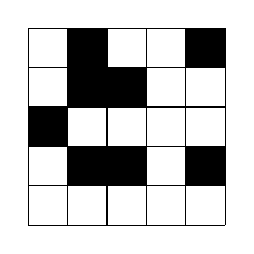
\begin{tikzpicture}[scale=0.5]
\fill[black] (1,1) rectangle (2,2);
\fill[black] (1,4) rectangle (2,5);
\fill[black] (4,1) rectangle (5,2);
\fill[black] (4,4) rectangle (5,5);
\fill[black] (1,3) rectangle (2,4);
\fill[black] (2,3) rectangle (3,4);
\fill[black] (2,1) rectangle (3,2);
\fill[black] (0,2) rectangle (1,3);
\draw (0,0) grid (5,5);
\end{tikzpicture}
\end{center}
chứa hai lưới con như vậy:
\begin{center}
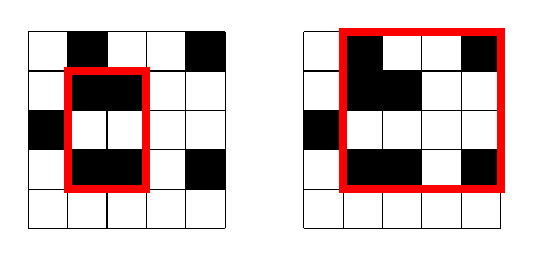
\begin{tikzpicture}[scale=0.5]
\fill[black] (1,1) rectangle (2,2);
\fill[black] (1,4) rectangle (2,5);
\fill[black] (4,1) rectangle (5,2);
\fill[black] (4,4) rectangle (5,5);
\fill[black] (1,3) rectangle (2,4);
\fill[black] (2,3) rectangle (3,4);
\fill[black] (2,1) rectangle (3,2);
\fill[black] (0,2) rectangle (1,3);
\draw (0,0) grid (5,5);

\fill[black] (7+1,1) rectangle (7+2,2);
\fill[black] (7+1,4) rectangle (7+2,5);
\fill[black] (7+4,1) rectangle (7+5,2);
\fill[black] (7+4,4) rectangle (7+5,5);
\fill[black] (7+1,3) rectangle (7+2,4);
\fill[black] (7+2,3) rectangle (7+3,4);
\fill[black] (7+2,1) rectangle (7+3,2);
\fill[black] (7+0,2) rectangle (7+1,3);
\draw (7+0,0) grid (7+5,5);

\draw[color=red,line width=1mm] (1,1) rectangle (3,4);
\draw[color=red,line width=1mm] (7+1,1) rectangle (7+5,5);
\end{tikzpicture}
\end{center}

Có một thuật toán thời gian $O(n^3)$ để giải quyết bài toán:
duyệt qua tất cả các cặp hàng $O(n^2)$ và cho mỗi cặp
$(a,b)$ tính số cột chứa
một ô vuông màu đen ở cả hai hàng trong thời gian $O(n)$.
Đoạn mã sau giả sử rằng $\texttt{color}[y][x]$
biểu thị màu ở hàng $y$ và cột $x$:
\begin{lstlisting}
int count = 0;
for (int i = 0; i < n; i++) {
    if (color[a][i] == 1 && color[b][i] == 1) count++;
}
\end{lstlisting}
Sau đó, những cột đó
chiếm $\texttt{count}(\texttt{count}-1)/2$ lưới con có các góc màu đen,
bởi vì chúng ta có thể chọn bất kỳ hai trong số chúng để tạo thành một lưới con.

Để tối ưu hóa thuật toán này, chúng ta chia lưới thành các khối
cột sao cho mỗi khối bao gồm $N$
cột liên tiếp. Sau đó, mỗi hàng được lưu trữ dưới dạng
một danh sách các số $N$ bit mô tả màu sắc
của các ô vuông. Bây giờ chúng ta có thể xử lý $N$ cột cùng một lúc
sử dụng các phép toán bit. Trong đoạn mã sau,
$\texttt{color}[y][k]$ biểu diễn
một khối $N$ màu dưới dạng các bit.
\begin{lstlisting}
int count = 0;
for (int i = 0; i <= n/N; i++) {
    count += __builtin_popcount(color[a][i]&color[b][i]);
}
\end{lstlisting}
Thuật toán kết quả hoạt động trong thời gian $O(n^3/N)$.

Chúng tôi đã tạo một lưới ngẫu nhiên có kích thước $2500 \times 2500$
và so sánh cách triển khai ban đầu và tối ưu hóa bit.
Trong khi mã ban đầu mất $29.6$ giây,
phiên bản tối ưu hóa bit chỉ mất $3.1$ giây
với $N=32$ (các số \texttt{int}) và $1.7$ giây
với $N=64$ (các số \texttt{long long}).

\section{Quy hoạch động}

Các phép toán bit cung cấp một cách hiệu quả và thuận tiện
để triển khai các thuật toán quy hoạch động
mà các trạng thái của chúng chứa các tập hợp con của các phần tử,
bởi vì các trạng thái như vậy có thể được lưu trữ dưới dạng các số nguyên.
Tiếp theo chúng ta thảo luận về các ví dụ về việc kết hợp
các phép toán bit và quy hoạch động.

\subsubsection{Lựa chọn tối ưu}

Ví dụ đầu tiên, hãy xem xét bài toán sau:
Chúng ta được cho giá của $k$ sản phẩm
trong $n$ ngày, và chúng ta muốn mua mỗi sản phẩm
đúng một lần.
Tuy nhiên, chúng ta chỉ được phép mua nhiều nhất một sản phẩm
trong một ngày.
Tổng giá tối thiểu là bao nhiêu?
Ví dụ, hãy xem xét kịch bản sau ($k=3$ và $n=8$):
\begin{center}
\begin{tikzpicture}[scale=.65]
    \draw (0, 0) grid (8,3);
    \node at (-2.5,2.5) {sản phẩm 0};
    \node at (-2.5,1.5) {sản phẩm 1};
    \node at (-2.5,0.5) {sản phẩm 2};

    \foreach \x in {0,...,7}
        {\node at (\x+0.5,3.5) {\x};}
    \foreach \x/\v in {0/6,1/9,2/5,3/2,4/8,5/9,6/1,7/6}
        {\node at (\x+0.5,2.5) {\v};}
    \foreach \x/\v in {0/8,1/2,2/6,3/2,4/7,5/5,6/7,7/2}
        {\node at (\x+0.5,1.5) {\v};}
    \foreach \x/\v in {0/5,1/3,2/9,3/7,4/3,5/5,6/1,7/4}
        {\node at (\x+0.5,0.5) {\v};}
\end{tikzpicture}
\end{center}
Trong kịch bản này, tổng giá tối thiểu là $5$:
\begin{center}
\begin{tikzpicture}[scale=.65]
    \fill [color=lightgray] (1, 1) rectangle (2, 2);
    \fill [color=lightgray] (3, 2) rectangle (4, 3);
    \fill [color=lightgray] (6, 0) rectangle (7, 1);
    \draw (0, 0) grid (8,3);
    \node at (-2.5,2.5) {sản phẩm 0};
    \node at (-2.5,1.5) {sản phẩm 1};
    \node at (-2.5,0.5) {sản phẩm 2};

    \foreach \x in {0,...,7}
        {\node at (\x+0.5,3.5) {\x};}
    \foreach \x/\v in {0/6,1/9,2/5,3/2,4/8,5/9,6/1,7/6}
        {\node at (\x+0.5,2.5) {\v};}
    \foreach \x/\v in {0/8,1/2,2/6,3/2,4/7,5/5,6/7,7/2}
        {\node at (\x+0.5,1.5) {\v};}
    \foreach \x/\v in {0/5,1/3,2/9,3/7,4/3,5/5,6/1,7/4}
        {\node at (\x+0.5,0.5) {\v};}
\end{tikzpicture}
\end{center}

Gọi $\texttt{price}[x][d]$ là giá của sản phẩm $x$
vào ngày $d$.
Ví dụ, trong kịch bản trên $\texttt{price}[2][3] = 7$.
Sau đó, gọi $\texttt{total}(S,d)$ là tổng giá
tối thiểu để mua một tập hợp con $S$ các sản phẩm trước ngày $d$.
Sử dụng hàm này, lời giải cho bài toán là
$\texttt{total}(\{0 \ldots k-1\},n-1)$.

Đầu tiên, $\texttt{total}(\emptyset,d) = 0$,
bởi vì không mất gì để mua một tập hợp rỗng,
và $\texttt{total}(\{x\},0) = \texttt{price}[x][0]$,
bởi vì có một cách để mua một sản phẩm vào ngày đầu tiên.
Sau đó, có thể sử dụng công thức đệ quy sau:
\begin{equation*}
\begin{split}
\texttt{total}(S,d) = \min( & \texttt{total}(S,d-1), \\
& \min_{x \in S} (\texttt{total}(S \setminus x,d-1)+\texttt{price}[x][d]))
\end{split}
\end{equation*}
Điều này có nghĩa là chúng ta hoặc không mua sản phẩm nào vào ngày $d$
hoặc mua một sản phẩm $x$ thuộc $S$.
Trong trường hợp thứ hai, chúng ta loại bỏ $x$ khỏi $S$ và cộng
giá của $x$ vào tổng giá.

Bước tiếp theo là tính các giá trị của hàm
sử dụng quy hoạch động.
Để lưu trữ các giá trị hàm, chúng ta khai báo một mảng
\begin{lstlisting}
int total[1<<K][N];
\end{lstlisting}
trong đó $K$ và $N$ là các hằng số đủ lớn.
Chiều thứ nhất của mảng tương ứng với một
biểu diễn bit của một tập hợp con.

Đầu tiên, các trường hợp $d=0$ có thể được xử lý như sau:
\begin{lstlisting}
for (int x = 0; x < k; x++) {
    total[1<<x][0] = price[x][0];
}
\end{lstlisting}
Sau đó, công thức đệ quy chuyển thành đoạn mã sau:
\begin{lstlisting}
for (int d = 1; d < n; d++) {
    for (int s = 0; s < (1<<k); s++) {
        total[s][d] = total[s][d-1];
        for (int x = 0; x < k; x++) {
            if (s&(1<<x)) {
                total[s][d] = min(total[s][d],
                                    total[s^(1<<x)][d-1]+price[x][d]);
            }
        }
    }
}
\end{lstlisting}
Độ phức tạp thời gian của thuật toán là $O(n 2^k k)$.

\subsubsection{Từ hoán vị đến tập hợp con}

Sử dụng quy hoạch động, thường có thể
thay đổi một vòng lặp qua các hoán vị thành
một vòng lặp qua các tập hợp con\footnote{Kỹ thuật này được giới thiệu vào năm 1962
bởi M. Held và R. M. Karp \cite{hel62}.}.
Lợi ích của việc này là
$n!$, số lượng các hoán vị,
lớn hơn nhiều so với $2^n$, số lượng các tập hợp con.
Ví dụ, nếu $n=20$, thì
$n! \approx 2.4 \cdot 10^{18}$ và $2^n \approx 10^6$.
Do đó, với một số giá trị của $n$,
chúng ta có thể duyệt qua các tập hợp con một cách hiệu quả nhưng không thể duyệt qua các hoán vị.

Ví dụ, hãy xem xét bài toán sau:
Có một thang máy với trọng lượng tối đa là $x$,
và $n$ người có trọng lượng đã biết
muốn đi từ tầng trệt
lên tầng trên cùng.
Số chuyến đi tối thiểu cần thiết là bao nhiêu
nếu mọi người vào thang máy theo một thứ tự tối ưu?

Ví dụ, giả sử rằng $x=10$, $n=5$
và các trọng lượng như sau:
\begin{center}
\begin{tabular}{ll}
người & trọng lượng \\
\hline
0 & 2 \\
1 & 3 \\
2 & 3 \\
3 & 5 \\
4 & 6 \\
\end{tabular}
\end{center}
Trong trường hợp này, số chuyến đi tối thiểu là 2.
Một thứ tự tối ưu là $\{0,2,3,1,4\}$,
chia mọi người thành hai chuyến đi:
đầu tiên là $\{0,2,3\}$ (tổng trọng lượng 10),
và sau đó là $\{1,4\}$ (tổng trọng lượng 9).

Bài toán có thể được giải quyết dễ dàng trong thời gian $O(n! n)$
bằng cách thử tất cả các hoán vị có thể có của $n$ người.
Tuy nhiên, chúng ta có thể sử dụng quy hoạch động để có được
một thuật toán hiệu quả hơn với thời gian $O(2^n n)$.
Ý tưởng là tính toán cho mỗi tập hợp con của mọi người
hai giá trị: số chuyến đi tối thiểu cần thiết và
trọng lượng tối thiểu của những người đi trong nhóm cuối cùng.

Gọi $\texttt{weight}[p]$ là trọng lượng của
người $p$.
Chúng ta định nghĩa hai hàm:
$\texttt{rides}(S)$ là số chuyến đi tối thiểu
cho một tập hợp con $S$,
và $\texttt{last}(S)$ là trọng lượng tối thiểu
của chuyến đi cuối cùng.
Ví dụ, trong kịch bản trên
\[ \texttt{rides}(\{1,3,4\})=2 \hspace{10px} \textrm{và}
\hspace{10px} \texttt{last}(\{1,3,4\})=5,\]
bởi vì các chuyến đi tối ưu là $\{1,4\}$ và $\{3\}$,
và chuyến đi thứ hai có trọng lượng 5.
Tất nhiên, mục tiêu cuối cùng của chúng ta là tính toán giá trị
của $\texttt{rides}(\{0 \ldots n-1\})$.

Chúng ta có thể tính các giá trị
của các hàm một cách đệ quy và sau đó áp dụng
quy hoạch động.
Ý tưởng là duyệt qua tất cả mọi người
thuộc $S$ và chọn một cách tối ưu
người cuối cùng $p$ vào thang máy.
Mỗi lựa chọn như vậy tạo ra một bài toán con
cho một tập hợp con nhỏ hơn của mọi người.
Nếu $\texttt{last}(S \setminus p)+\texttt{weight}[p] \le x$,
chúng ta có thể thêm $p$ vào chuyến đi cuối cùng.
Ngược lại, chúng ta phải dành một chuyến đi mới
ban đầu chỉ chứa $p$.

Để triển khai quy hoạch động,
chúng ta khai báo một mảng
\begin{lstlisting}
pair<int,int> best[1<<N];
\end{lstlisting}
chứa cho mỗi tập hợp con $S$
một cặp $(\texttt{rides}(S),\texttt{last}(S))$.
Chúng ta đặt giá trị cho một nhóm rỗng như sau:
\begin{lstlisting}
best[0] = {1,0};
\end{lstlisting}
Sau đó, chúng ta có thể điền vào mảng như sau:

\begin{lstlisting}
for (int s = 1; s < (1<<n); s++) {
    // gia tri ban dau: can n+1 chuyen di
    best[s] = {n+1,0};
    for (int p = 0; p < n; p++) {
        if (s&(1<<p)) {
            auto option = best[s^(1<<p)];
            if (option.second+weight[p] <= x) {
                // them p vao mot chuyen di da co
                option.second += weight[p];
            } else {
                // danh mot chuyen di moi cho p
                option.first++;
                option.second = weight[p];
            }
            best[s] = min(best[s], option);
        }
    }
}
\end{lstlisting}
Lưu ý rằng vòng lặp trên đảm bảo rằng
với bất kỳ hai tập hợp con $S_1$ và $S_2$
nào sao cho $S_1 \subset S_2$, chúng ta xử lý $S_1$ trước $S_2$.
Do đó, các giá trị quy hoạch động được tính toán theo
thứ tự đúng.

\subsubsection{Đếm tập hợp con}

Bài toán cuối cùng của chúng ta trong chương này như sau:
Cho $X=\{0 \ldots n-1\}$, và mỗi tập hợp con $S \subset X$
được gán một số nguyên $\texttt{value}[S]$.
Nhiệm vụ của chúng ta là tính toán cho mỗi $S$
\[\texttt{sum}(S) = \sum_{A \subset S} \texttt{value}[A],\]
tức là, tổng các giá trị của các tập hợp con của $S$.

Ví dụ, giả sử rằng $n=3$ và các giá trị như sau:
\begin{multicols}{2}
\begin{itemize}
\item $\texttt{value}[\emptyset] = 3$
\item $\texttt{value}[\{0\}] = 1$
\item $\texttt{value}[\{1\}] = 4$
\item $\texttt{value}[\{0,1\}] = 5$
\item $\texttt{value}[\{2\}] = 5$
\item $\texttt{value}[\{0,2\}] = 1$
\item $\texttt{value}[\{1,2\}] = 3$
\item $\texttt{value}[\{0,1,2\}] = 3$
\end{itemize}
\end{multicols}
Trong trường hợp này, ví dụ,
\begin{equation*}
\begin{split}
\texttt{sum}(\{0,2\}) &= \texttt{value}[\emptyset]+\texttt{value}[\{0\}]+\texttt{value}[\{2\}]+\texttt{value}[\{0,2\}] \\ 
                      &= 3 + 1 + 5 + 1 = 10.
\end{split}
\end{equation*}

Vì có tổng cộng $2^n$ tập hợp con,
một giải pháp khả thi là duyệt qua tất cả
các cặp tập hợp con trong thời gian $O(2^{2n})$.
Tuy nhiên, bằng cách sử dụng quy hoạch động, chúng ta
có thể giải quyết bài toán trong thời gian $O(2^n n)$.
Ý tưởng là tập trung vào các tổng mà các
phần tử có thể bị loại bỏ khỏi $S$ bị hạn chế.

Gọi $\texttt{partial}(S,k)$ là tổng các
giá trị của các tập hợp con của $S$ với hạn chế
rằng chỉ có các phần tử $0 \ldots k$
mới có thể bị loại bỏ khỏi $S$.
Ví dụ,
\[\texttt{partial}(\{0,2\},1)=\texttt{value}[\{2\}]+\texttt{value}[\{0,2\}],\]
bởi vì chúng ta chỉ có thể loại bỏ các phần tử $0 \ldots 1$.
Chúng ta có thể tính các giá trị của \texttt{sum} bằng cách sử dụng
các giá trị của \texttt{partial}, bởi vì
\[\texttt{sum}(S) = \texttt{partial}(S,n-1).\]
Các trường hợp cơ sở cho hàm là
\[\texttt{partial}(S,-1)=\texttt{value}[S],\]
bởi vì trong trường hợp này không có phần tử nào có thể bị loại bỏ khỏi $S$.
Sau đó, trong trường hợp tổng quát, chúng ta có thể sử dụng công thức đệ quy sau:
\begin{equation*}
    \texttt{partial}(S,k) = \begin{cases}
               \texttt{partial}(S,k-1) & k \notin S \\
               \texttt{partial}(S,k-1) + \texttt{partial}(S \setminus \{k\},k-1) & k \in S
           \end{cases}
\end{equation*}
Ở đây chúng ta tập trung vào phần tử $k$.
Nếu $k \in S$, chúng ta có hai lựa chọn: chúng ta có thể giữ $k$ trong $S$
hoặc loại bỏ nó khỏi $S$.

Có một cách đặc biệt thông minh để triển khai việc
tính toán các tổng. Chúng ta có thể khai báo một mảng
\begin{lstlisting}
int sum[1<<N];
\end{lstlisting}
sẽ chứa tổng của mỗi tập hợp con.
Mảng được khởi tạo như sau:
\begin{lstlisting}
for (int s = 0; s < (1<<n); s++) {
    sum[s] = value[s];
}
\end{lstlisting}
Sau đó, chúng ta có thể điền vào mảng như sau:
\begin{lstlisting}
for (int k = 0; k < n; k++) {
    for (int s = 0; s < (1<<n); s++) {
        if (s&(1<<k)) sum[s] += sum[s^(1<<k)];
    }
}
\end{lstlisting}
Đoạn mã này tính các giá trị của $\texttt{partial}(S,k)$
cho $k=0 \ldots n-1$ vào mảng \texttt{sum}.
Vì $\texttt{partial}(S,k)$ luôn dựa trên
$\texttt{partial}(S,k-1)$, chúng ta có thể tái sử dụng mảng
\texttt{sum}, mang lại một cách triển khai rất hiệu quả.